\chapter{วิศวกรรมเฟิร์มแวร์ไมโครคอนโทรลเลอร์และการแก้ไขปัญหาเชิงลึก}
\label{chap:firmware}

ความสำเร็จของการประยุกต์ใช้ระบบสมองกลฝังตัวในแปลงเกษตรกรรมขึ้นอยู่กับความเสถียรของเฟิร์มแวร์ ความสามารถในการรองรับข้อผิดพลาดของสัญญาณฮาร์ดแวร์ และการประมวลผลข้อมูลทางฟิสิกส์ได้อย่างถูกต้องแม่นยำ บทนี้นำเสนอโครงสร้างเฟิร์มแวร์ ระบบคำนวณทางปฐพีวิทยา และกระบวนการวิเคราะห์หาสาเหตุเชิงลึก (Root Cause Analysis หรือ RCA) ในการแก้ไขปัญหาทางวิศวกรรมที่เกิดขึ้นระหว่างการพัฒนาจริง

\section{โครงสร้างเฟิร์มแวร์และการจัดการทรัพยากรบนระบบ PlatformIO}

โครงการได้รับการพัฒนาภายใต้สภาพแวดล้อม \textbf{PlatformIO}\index{PlatformIO} ร่วมกับเฟรมเวิร์ก Arduino บนระบบปฏิบัติการ macOS โดยมีการจัดโครงสร้างซอฟต์แวร์แบบโมดูลาร์ (Modular Architecture) เพื่อแยกส่วนควบคุมฮาร์ดแวร์ออกจากลอจิกการตัดสินใจทางเกษตรกรรม

\begin{agribox}{โมดูลหลักของเฟิร์มแวร์ระบบ JC -AgriTech + AI}
    \begin{itemize}
        \item \textbf{PinConfigs.h} นิยามการจัดสรรขาสัญญาณไมโครคอนโทรลเลอร์ ESP32-S3\index{ESP32-S3} ให้ตรงกับวงจรจริง
        \item \textbf{UserConfigs.h} รวบรวมพารามิเตอร์การตั้งค่าของผู้ใช้ เช่น แอดเดรสเซนเซอร์ ค่าการคาลิเบรต ADC ข้อมูลเครือข่าย Wi-Fi และ IP ปลายทาง
        \item \textbf{AgriSensors.cpp} ไดรเวอร์ระดับล่างสำหรับสื่อสารกับ SHT45, BH1750, Soil Stick และเซนเซอร์ 7-in-1 Modbus RTU\index{Modbus RTU}
        \item \textbf{DisplayManager.cpp} ไดรเวอร์กราฟิกและระบบแสดงผลหน้าปัดบนจอ LCD 3.5 นิ้ว ผ่านไลบรารี LovyanGFX\index{LovyanGFX}
        \item \textbf{CloudDataManager.cpp} ระบบจัดการเครือข่ายไร้สาย ซิงค์เวลามาตรฐานโลก NTP และสตรีมข้อมูลทาง HTTP/HTTPS
        \item \textbf{main.cpp} ลูปควบคุมหลักที่ประสานการอ่านค่า การตัดสินใจเปิด-ปิดรีเลย์ และการอัปเดตหน้าปัด
    \end{itemize}
\end{agribox}

\section{การคำนวณพารามิเตอร์ทางปฐพีวิทยาและสภาวะบรรยากาศ}

นอกจากค่าพื้นฐานที่อ่านได้จากเซนเซอร์ ระบบยังฝังอัลกอริทึมการคำนวณดัชนีชี้วัดทางสรีรวิทยาของพืชที่มีความสำคัญสูงต่อการจัดการน้ำและการระบายความร้อน ได้แก่

\subsection{จุดน้ำค้างในบรรยากาศ}
จุดน้ำค้าง (Dew Point Temperature หรือ $T_d$) คำนวณผ่านสมการมักนุส-เทเทนส์ (Magnus-Tetens Equation) ซึ่งมีความแม่นยำสูงในช่วงอุณหภูมิ $0$ ถึง $60\ ^\circ\text{C}$

\begin{equation}
    \alpha(T, \text{RH}) = \frac{a \cdot T}{b + T} + \ln\left(\frac{\text{RH}}{100}\right), \quad T_d = \frac{b \cdot \alpha(T, \text{RH})}{a - \alpha(T, \text{RH})}
    \label{eq:dew_point}
\end{equation}

โดยกำหนดค่าสัมประสิทธิ์เชิงประจักษ์ $a = 17.27$ และ $b = 237.7\ ^\circ\text{C}$

\subsection{แรงดึงระเหยน้ำของบรรยากาศและการประเมินสภาวะทางสรีรวิทยา}
แรงดึงระเหยน้ำ (Vapor Pressure Deficit หรือ VPD) มีหน่วยเป็นกิโลปาสกาล (kPa) เป็นตัวแปรที่บ่งบอกความสามารถในการคายน้ำและการเปิด-ปิดปากใบของพืช ค่า VPD คำนวณจากผลต่างระหว่างความดันไอน้ำอิ่มตัว ($VP_{\text{sat}}$) และความดันไอน้ำจริง ($VP_{\text{act}}$)

\begin{equation}
    VP_{\text{sat}} = 0.61078 \exp\left(\frac{17.27 \cdot T}{T + 237.3}\right), \quad VP_{\text{act}} = VP_{\text{sat}} \times \left(\frac{\text{RH}}{100}\right)
    \label{eq:vpd_sat}
\end{equation}
\begin{equation}
    \text{VPD} = VP_{\text{sat}} - VP_{\text{act}}
    \label{eq:vpd}
\end{equation}

\begin{table}[htbp]
    \caption{เกณฑ์การประเมินสภาวะความเครียดของพืชตามระดับความดันไอน้ำอิ่มตัว (VPD Index)}
    \label{tab:vpd_criteria}
    \begin{tabularx}{\textwidth}{p{3.0cm}p{3.2cm}Y}
        \toprule
        \textbf{ช่วงค่า VPD (kPa)} & \textbf{สภาวะบรรยากาศ} & \textbf{ผลกระทบทางสรีรวิทยาของพืชและการจัดการ} \\
        \midrule
        $< 0.40$ & ชื้นจัดเกินไป (Under-transpiration) & เสี่ยงต่อการเกิดโรคเชื้อรา ปากใบไม่ระบายน้ำ พืชขาดแคลเซียม \\
        $0.40 - 0.80$ & สภาวะอ่อนโยน (Propagation Zone) & เหมาะสำหรับระยะเพาะเมล็ด อนุบาลต้นกล้า หรือแปลงปักชำ \\
        $\mathbf{0.80 - 1.20}$ & \textbf{ช่วงเหมาะสมที่สุด (Optimal Zone)} & \textbf{อัตราการสังเคราะห์แสงและการดูดซึมธาตุอาหารสูงสุด} \\
        $1.20 - 1.60$ & ค่อนข้างแห้ง (Mild Water Stress) & เหมาะสำหรับพืชทนแล้ง หรือการควบคุมความหวานในผลไม้ \\
        $> 1.60$ & แห้งแล้งจัด (Severe Water Stress) & ปากใบปิดสนิท พืชเหี่ยวเฉา ชะงักการเจริญเติบโต ต้องพ่นหมอก \\
        \bottomrule
    \end{tabularx}
\end{table}

\section{สถาปัตยกรรมแบบจำลองสถานะของเฟิร์มแวร์ (Firmware State Machine)}

การประมวลผลภายในไมโครคอนโทรลเลอร์ ESP32-S3 ถูกควบคุมด้วยระบบ Finite State Machine (FSM) ที่มีรอบการทำงานอย่างเป็นระบบ เพื่อให้มั่นใจว่าการอ่านเซนเซอร์ การคำนวณทางฟิสิกส์ การเรนเดอร์หน้าปัด และการสตรีมข้อมูลขึ้นเซิร์ฟเวอร์ดำเนินไปอย่างราบรื่นโดยไม่บล็อกการทำงานของลูปควบคุมหลัก

\begin{figure}[htbp]
\centering
\resizebox{0.82\textwidth}{!}{
\begin{tikzpicture}[
    node distance=1.3cm and 1.5cm,
    state/.style={rectangle, draw=rbruNavy, fill=white, thick, rounded corners=4pt, align=center, minimum height=1.0cm, minimum width=3.2cm, drop shadow={opacity=0.15}},
    startstate/.style={rectangle, draw=rbruGold!90!black, fill=rbruNavy, thick, rounded corners=4pt, text=white, align=center, minimum height=1.0cm, minimum width=3.0cm},
    arrow/.style={draw=rbruNavy, -latex', thick}
]
    % Symmetrical balancing coordinate on the left
    \coordinate (left_balance) at (-2.8,0);

    \node[startstate] (boot) {\textbf{BOOT \& HARDWARE INIT}\\\footnotesize Flash 8MB DIO $\cdot$ GPIO Assign};
    \node[state, right=1.4cm of boot] (probe) {\textbf{I2C DIAGNOSTIC PROBE}\\\footnotesize Scan SDA=9, SCL=8 (0x23, 0x44)};
    \node[state, below=1.2cm of probe] (read) {\textbf{SENSOR TELEMETRY CYCLE}\\\footnotesize Read SHT45, Dome, Stick, 7-in-1};
    \node[state, left=1.4cm of read] (physics) {\textbf{PHYSICS MATH ENGINE}\\\footnotesize Dew Point, Solar Radiation, VPD};
    \node[state, below=1.2cm of physics] (disp) {\textbf{LOVYANGFX UI REFRESH}\\\footnotesize ST7796 IPS Invert $\cdot$ Thai Bitmap};
    \node[state, right=1.4cm of disp] (net) {\textbf{ASYNC TELEMETRY DISPATCH}\\\footnotesize Non-blocking POST $\cdot$ NTP Sync};

    \draw[arrow] (boot) -- (probe);
    \draw[arrow] (probe) -- (read);
    \draw[arrow] (read) -- (physics);
    \draw[arrow] (physics) -- (disp);
    \draw[arrow] (disp) -- (net);
    \draw[arrow] (net.east) -- ++(0.8,0) |- (read.east) node[near end, right, font=\scriptsize\color{rbruSlate}] {Every 15s Loop};

    % Draw invisible balance on left to keep diagram exactly centered
    \path (physics.west) ++(-1.6,0) coordinate (lb);
    \path (lb) node {};
\end{tikzpicture}
}
\caption{แผนผังสถานะการทำงานของระบบเฟิร์มแวร์ JC -AgriTech + AI (Firmware FSM)}
\label{fig:firmware_fsm}
\end{figure}

\section{การวิเคราะห์สาเหตุเชิงลึกและการแก้ไขปัญหาหน้าจอมืดสนิท}

ในขั้นตอนการติดตั้งโปรแกรมเบื้องต้น พบปัญหาหน้าจอ LCD แสดงผลเป็นจอมืดสนิท ไม่มีข้อความหรือกราฟิกใดๆ ปรากฏ กระบวนการสืบสวนเชิงลึกพบสาเหตุสำคัญ 2 ประการที่ซ้อนทับกันอยู่

\begin{figure}[htbp]
    \centering
    \begin{minipage}[b]{0.48\textwidth}
        \centering
        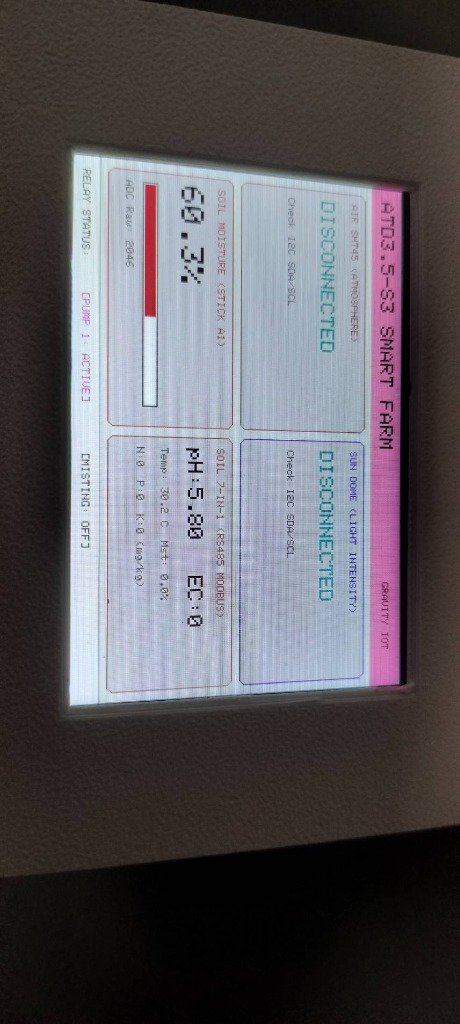
\includegraphics[height=5.2cm,width=\textwidth,keepaspectratio]{figures/black_screen_issue.jpg}
        \caption{สภาวะจอดำจากขาแบล็กไลต์ขัดแย้งกับ Flash}
        \label{fig:black_screen_issue}
    \end{minipage}
    \hfill
    \begin{minipage}[b]{0.48\textwidth}
        \centering
        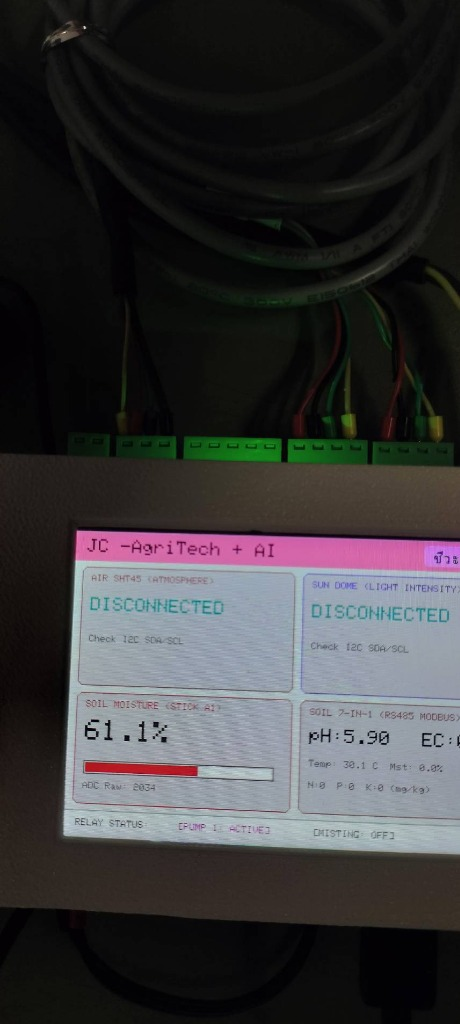
\includegraphics[height=5.2cm,width=\textwidth,keepaspectratio]{figures/lcd_screen.jpg}
        \caption{หน้าจอติดสว่างสมบูรณ์แบบหลังการทำ RCA}
        \label{fig:lcd_screen_fixed}
    \end{minipage}
\end{figure}

\begin{workedbox}{การสืบสวนปัญหาหน้าจอดำและการแก้ปัญหาทางวิศวกรรม (Root Cause Analysis)}
    \begin{enumerate}
        \item \textbf{การขัดแย้งของขาสัญญาณควบคุมไฟหน้าจอ (Backlight Pin Conflict):}
        จากการตรวจสอบวงจรไฟฟ้าของบอร์ด ATD3.5-S3 พบว่าขาควบคุมไฟส่องสว่างด้านหลังจอภาพ (LCD Backlight) ต่ออยู่กับขา \textbf{GPIO38} (หรือ GPIO3 บนบอร์ดบางล็อต) ของ ESP32-S3 แต่ในโค้ดเดิมได้นิยามให้รีเลย์ตัวที่ 2 เป็นขานี้ และสั่งคำสั่ง \texttt{digitalWrite(PIN, LOW)} ในฟังก์ชัน \texttt{setup()} ส่งผลให้สัญญาณไฟ Backlight ถูกตัดไฟอย่างถาวร
        \item \textbf{การบูตรีเซ็ตวนรอบจากขนาดหน่วยความจำแฟลช (Flash Boot Loop):}
        บอร์ด ATD3.5-S3 ติดตั้งชิป Flash ขนาด 8 MB แต่คอนฟิกดั้งเดิมใน \texttt{platformio.ini} กำหนดขนาดไว้ที่ 16 MB QIO ส่งผลให้บูตโหลดเดอร์เกิดข้อผิดพลาด \texttt{flash\_ret == ESP\_OK} และสั่งรีเซ็ตชิปตลอดเวลา
    \end{enumerate}
    \textbf{แนวทางแก้ไข:}
    แก้ไขการจัดสรรขารีเลย์บน Farm1 Shield ให้ถูกต้อง สั่งเปิดไฟจอด้วยคำสั่ง \texttt{digitalWrite(LCD\_BL\_PIN, HIGH)} พร้อมปรับแต่ง \texttt{platformio.ini} ให้กำหนดโหมด \texttt{flash\_size = 8MB}, \texttt{flash\_mode = dio} และตารางพาร์ติชัน \texttt{default\_8MB.csv} ส่งผลให้ระบบบูตขึ้นทำงานได้อย่างสมบูรณ์
\end{workedbox}

\section{การสืบสวนสัญญาณ I2C สลับพินด้วย Diagnostic Scanner}

ภายหลังหน้าจอติดสว่าง พบปัญหาเซนเซอร์ SHT45 และเซนเซอร์โดมตะวันแสดงสถานะ \texttt{DISCONNECTED} บนจอภาพ เพื่อหลีกเลี่ยงการรื้อสายไฟหรือตัดต่อวงจรในแปลงปลูก ทีมวิจัยได้เขียนสคริปต์สแกนสัญญาณ I2C ฮาร์ดแวร์แบบ Real-time ผลการทดสอบพบว่า

\begin{pythonbox}[ซอฟต์แวร์สแกนค้นหาแอดเดรสบนบัส I2C (I2C Bus Scanner)]
void scanI2CBus(int sdaPin, int sclPin) {
    Wire.begin(sdaPin, sclPin);
    Serial.printf("Scanning I2C on SDA=GPIO%d, SCL=GPIO%d...\n", sdaPin, sclPin);
    int deviceCount = 0;
    for (uint8_t addr = 1; addr < 127; addr++) {
        Wire.beginTransmission(addr);
        if (Wire.endTransmission() == 0) {
            Serial.printf("  Found device at address: 0x%02X\n", addr);
            deviceCount++;
        }
    }
    Serial.printf("Total devices detected: %d\n", deviceCount);
}
\end{pythonbox}

ผลการสแกนเชิงประจักษ์:
\begin{itemize}
    \item เมื่อกำหนดพินเริ่มต้น SDA=GPIO8, SCL=GPIO9 ตรวจพบเฉพาะแอดเดรส \texttt{0x51} (ไอซีนาฬิกา RTC PCF8563 บนบอร์ดหลัก)
    \item เมื่อสลับพินเป็น \textbf{SDA=GPIO9, SCL=GPIO8} ระบบตรวจพบแอดเดรส \textbf{\texttt{0x23} (โดมตะวัน BH1750)} และ \textbf{\texttt{0x44} (เซนเซอร์ SHT45)} พร้อมกันในทันที
\end{itemize}

สิ่งนี้ยืนยันว่าการต่อสายไฟของเซนเซอร์บนเทอร์มินัลบล็อกคือ สายสีเหลืองต่ออยู่กับขา 4 (GPIO9) และสายสีเขียวต่ออยู่กับขา 3 (GPIO8) การปรับแต่งค่าในซอฟต์แวร์ให้ตรงกับการต่อสายจริงช่วยประหยัดเวลาและป้องกันความเสียหายที่อาจเกิดขึ้นกับขั้วต่อฮาร์ดแวร์

\section{การออกแบบเลย์เอาต์หน้าปัดและการสังเคราะห์บิตแมปภาษาไทย}

หน้าจอแสดงผลขนาด 3.5 นิ้ว ได้รับการออกแบบเลย์เอาต์เป็น 4 การ์ดอิสระ แสดงข้อมูลสภาพอากาศ แสงสว่าง ดินผิวดิน และดินลึก เพื่อความสวยงามและคมชัดสูงสุด ระบบได้แก้ไขปัญหาพาเนลจอ ST7796 IPS แสดงผลสีกลับด้าน (Color Inversion) โดยการเปิดแฟล็ก \texttt{cfg.invert = true;} ภายในคลาสไดรเวอร์ LovyanGFX ส่งผลให้ได้ธีม Dark Mode สีดำมืดสนิท คอนทราสต์สูง และสบายตา

นอกจากนี้ เพื่อให้หน้าจอแสดงเอกลักษณ์ของผู้วิจัย ได้มีการสังเคราะห์ฟอนต์บิตแมปภาษาไทยความละเอียดสูงขนาด $84 \times 18$ พิกเซล คำว่า \textbf{"ชีวะ  ทัศนา"} จัดวางบนกล่องสีเขียวมรกตที่มุมขวาบนของหน้าปัดเคียงคู่กับหัวข้อหลัก \textbf{"JC -AgriTech + AI"} แสดงผลได้อย่างสมบูรณ์แบบโดยไม่ต้องพึ่งพาชิปฟอนต์ภายนอก

\section{การปรับปรุงส่วนต่อประสานผู้ใช้แบบสัมผัสและสถาปัตยกรรมสามภาษา}

การยกระดับประสบการณ์ของผู้ใช้งาน (User Experience หรือ UX) ในแปลงเกษตรกรรมมีความสำคัญอย่างยิ่งต่อความถูกต้องในการติดตามสภาวะแปลงปลูก ในระยะพัฒนาขั้นสูง ระบบได้รับการปรับปรุงส่วนต่อประสานผู้ใช้บนหน้าจอสัมผัส IPS ขนาด 3.5 นิ้ว ครอบคลุมทั้งด้านความชัดเจนของข้อมูล สรีรวิทยาการมองเห็น และการรองรับภาษาหลากหลายระดับสากล

\subsection{การจัดระเบียบข้อมูลบนการ์ดภาพรวมและสัญลักษณ์ทางฟิสิกส์}

ในหน้าต่างหลัก (Overview Page) ระบบได้รับการปรับโครงสร้างเลย์เอาต์การแสดงผลเพื่อเพิ่มความคลีนและความสบายตา (Clean and Modern Minimalism) โดยมีรายละเอียดการพัฒนาที่สำคัญดังนี้
\begin{enumerate}
    \item \textbf{การตัดข้อความสถานะในวงเล็บที่ไม่จำเป็นออก} เดิมทีหน้าจอมีการแสดงผลข้อความสถานะในวงเล็บ เช่น คำว่า [ชื้นสูง เสี่ยงเชื้อรา], [แดดร่ม/ครึ้ม พืชพักตัว], และคำแนะนำการกด [แตะดู] ทั้งสามภาษา ซึ่งทำให้หน้าจอดูแออัดและบดบังค่าสถิติหลัก เมื่อตัดข้อความดังกล่าวออก หน้าจอมีพื้นที่ว่างสำหรับแสดงผลตัวเลขด้วยฟอนต์ขนาดใหญ่ขึ้นอย่างชัดเจน
    \item \textbf{การจัดแถวคู่สำหรับอุณหภูมิและความชื้นสัมพัทธ์ในอากาศ} การ์ดสภาพอากาศได้รับการจัดวางค่าอุณหภูมิ ($^\circ\text{C}$) และความชื้นสัมพัทธ์ (\%RH) ให้อยู่ในแถวเดียวกันแบบสองคอลัมน์สมมาตร และย้ายค่าแรงดึงระเหยน้ำของบรรยากาศ VPD (kPa) ลงมาอยู่แถวด้านล่าง ทำให้ตัวเลขมีขนาดใหญ่ขึ้นและผู้ใช้สามารถกวาดสายตาอ่านค่าได้อย่างรวดเร็ว
    \item \textbf{การกำหนดหน่วยฟิสิกส์พลังงานรังสีดวงอาทิตย์เป็นตัวยก} ปรับเปลี่ยนการแสดงผลหน่วยวัดพลังงานรังสีดวงอาทิตย์จากการพิมพ์เป็นตัวอักษรธรรมดา W/m2 มาเป็นการใช้สัญลักษณ์ตัวยกที่ถูกต้องตามมาตรฐานสากลคือ $\text{W/m}^2$ (วัตต์ต่อตารางเมตร)
    \item \textbf{การระบุหน่วยวิศวกรรมสำหรับการ์ดธาตุอาหารดิน NPK} เพิ่มหน่วยวัดทางวิศวกรรมกำกับท้ายค่าไนโตรเจน ฟอสฟอรัส และโพแทสเซียมอย่างชัดเจนในหน่วย $\text{mg/kg}$ (มิลลิกรัมต่อกิโลกรัม)
    \item \textbf{ปุ่มเมนูนำทางแบบแยกสีเด่นชัด} แถบเมนูด้านล่างสุดของหน้าจอได้รับการปรับเปลี่ยนเป็นปุ่มกด 4 ปุ่มที่แยกขอบสีอย่างชัดเจน ได้แก่ ปุ่มภาพรวม (สีเขียวมรกต), ปุ่มข้อมูลและกราฟ (สีฟ้าไซแอน), ปุ่มควบคุมรีเลย์ (สีแดง), และปุ่มตั้งค่าระบบ (สีเหลืองทอง) ช่วยให้เกษตรกรสามารถใช้นิ้วสัมผัสสั่งการได้อย่างแม่นยำแม้ในสภาพแสงแดดจ้า
\end{enumerate}

\subsection{สถาปัตยกรรมระบบเรนเดอร์สามภาษาแบบไดนามิก}

เพื่อรองรับการใช้งานในระดับสากลและเกษตรกรทุกกลุ่ม ระบบฝังกลไกสลับภาษา 3 ภาษาแบบเรียลไทม์ (Tri-Lingual System) ประกอบด้วย ภาษาไทย (Thai), ภาษาอังกฤษ (English), และภาษาจีน (Chinese) ผ่านปุ่มสัมผัสที่มุมบนขวาของหน้าจอ
\begin{itemize}
    \item \textbf{ภาษาไทย (Thai)} ใช้ไฟล์ฟอนต์เวกเตอร์บิตแมปแบบกำหนดเอง \texttt{ThaiFontVLW.h} ฝังในหน่วยความจำ Flash ของ ESP32-S3 รองรับพยัญชนะ สระ และวรรณยุกต์ไทยครบถ้วนตามรหัสยูนิโค้ด
    \item \textbf{ภาษาจีน (Chinese)} เรียกใช้ชุดฟอนต์ฮั่นจื้อความเร็วสูง \texttt{\&fonts::efontCN\_14} ที่บรรจุในไลบรารี LovyanGFX
    \item \textbf{ภาษาอังกฤษ (English)} เรียกใช้ชุดฟอนต์แอสกีแบบบิตแมปความเร็วสูง
\end{itemize}
การสลับภาษาสามารถทำได้ทันทีเมื่อแตะสัมผัส โดยระบบจะวนลูปภาษา ภาษาไทย $\rightarrow$ English $\rightarrow$ Chinese $\rightarrow$ ภาษาไทย และเรนเดอร์ข้อความทั้งหมดใหม่ภายในเวลาไม่เกิน 50 มิลลิวินาทีโดยไม่ต้องรีเซ็ตไมโครคอนโทรลเลอร์

\section{ระบบแอนิเมชันเปิดเครื่อง 3 มิติและการเรนเดอร์กราฟิกเสมือนจริง}

เพื่อสร้างความประทับใจตั้งแต่เริ่มเปิดใช้งานเครื่อง ระบบได้รับการออกแบบลำดับแอนิเมชันเปิดเครื่อง (Boot Animation) สไตล์ 3D Pixar และไซไฟล้ำสมัย ด้วยการใช้ขุมพลังการประมวลผลกราฟิกของ LovyanGFX ร่วมกับชิป ESP32-S3 Dual-Core 240 MHz

\subsection{แบบจำลองการให้แสงเงาแบบบลินน์-ฟองบนหน่วยประมวลผลฝังตัว}

การสร้างภาพทรงกลม 3 มิติที่มีมิติความลึกเสมือนจริงโดยไม่ใช้ชิปประมวลผลกราฟิก (GPU) ภายนอก กระทำได้โดยการนำแบบจำลองแสงเงาทางฟิสิกส์แบบบลินน์-ฟอง (Blinn-Phong Illumination Model)\index{Blinn-Phong} มาเขียนเป็นลอจิกคณิตศาสตร์ในระดับพิกเซล ความสว่างรวม $I$ ที่ตกกระทบบนผิวทรงกลมคำนวณจากผลรวมของแสงแวดล้อม แสงสะท้อนแบบกระจาย และแสงสะท้อนตรงแบบสเปคิวลาร์

\begin{equation}
    I = I_{\text{ambient}} + I_{\text{diffuse}} \max(\mathbf{N} \cdot \mathbf{L}, 0) + I_{\text{specular}} \max(\mathbf{N} \cdot \mathbf{H}, 0)^\gamma
    \label{eq:blinn_phong}
\end{equation}

โดยที่ $\mathbf{N}$ คือเวกเตอร์แนวฉากหนึ่งหน่วยของพื้นผิวทรงกลมที่พิกัด $(x, y, z)$, $\mathbf{L}$ คือเวกเตอร์ทิศทางของแหล่งกำเนิดแสง, $\mathbf{V}$ คือเวกเตอร์มุมมองของผู้สังเกต, $\mathbf{H} = \frac{\mathbf{L} + \mathbf{V}}{\|\mathbf{L} + \mathbf{V}\|}$ คือเวกเตอร์กึ่งกลางทิศทาง (Halfway Vector), และ $\gamma$ คือค่าสัมประสิทธิ์ความมันวาวของพื้นผิว (Shininess Exponent)

\subsection{ลำดับแอนิเมชันเปิดเครื่อง 10 เฟส}

วงรอบการเปิดเครื่องถูกแบ่งออกเป็น 10 เฟสต่อเนื่องที่อัตราเฟรม 30 ภาพต่อวินาที ประกอบด้วย
\begin{enumerate}
    \item \textbf{เฟสที่ 1 ถึง 3 (เรดาร์และวงจรอิเล็กทรอนิกส์)} เส้นสแกนเนอร์และลายวงจรไฟฟ้าสีฟ้าไซแอนวิ่งกวาดทั่วหน้าจอ Dark Mode พร้อมจุดเชื่อมต่อที่กะพริบเป็นจังหวะ
    \item \textbf{เฟสที่ 4 ถึง 7 (ทรงกลม 3 มิติมหัศจรรย์)} การเรนเดอร์ทรงกลมแสง 3 มิติที่มีไฮไลต์แสงสะท้อนขยับหมุนอย่างนุ่มนวล ให้ความรู้สึกเสมือนวัตถุจริงลอยอยู่เหนือหน้าปัด
    \item \textbf{เฟสที่ 8 ถึง 10 (ตราสัญลักษณ์และเครดิตผู้วิจัย)} การปรากฏของโลโก้ข้อความตัวหนานูน \textbf{"JC AGRITecH+AI."} พร้อมเปล่งแสงนีออนล้อมรอบ และแสดงรายชื่อผู้วิจัยและพัฒนา \textbf{"ผศ.ดร.ชีวะ ทัศนา"} และ \textbf{"ผศ.ดร.จิรภัทร จันทมาลี"} ร่วมกับหลอดสถานะการโหลดข้อมูล (Shimmer Progress Bar) จาก 0\% สู่ 100\%
\end{enumerate}
เมื่อหลอดสถานะเต็ม 100\% ระบบจะสั่งล้างบัฟเฟอร์ภาพและสลับเข้าสู่หน้าจอภาพรวมหลัก (Overview Page) อย่างราบรื่นในทันที

\section{การสอบเทียบและปรับแต่งพารามิเตอร์เซนเซอร์วัดดิน 7-in-1 Modbus RS485}

เซนเซอร์วัดคุณสมบัติดินแบบแท่งโลหะมัลติโพรบ 7-in-1 สื่อสารผ่าน RS485 Modbus RTU เป็นอุปกรณ์ที่มีความทนทานสูง แต่การวัดปริมาณธาตุอาหารหลัก ไนโตรเจน (N), ฟอสฟอรัส (P), และโพแทสเซียม (K) ในเซนเซอร์ประเภทนี้ไม่ได้อาศัยขั้วไฟฟ้าเลือกจำเพาะไอออน (Ion-Selective Electrode หรือ ISE) โดยตรง หากแต่อาศัยการอนุมานทางอ้อมจากค่าความต้านทานไฟฟ้าและสภาพนำไฟฟ้าของสารละลายในดิน ส่งผลให้ค่าที่อ่านได้จากโรงงานมักมีความคลาดเคลื่อนต่ำกว่าความเป็นจริงในดินธรรมชาติ

\subsection{แบบจำลองการสอบเทียบเชิงเส้นทางปฐพีวิทยา}

เพื่อปรับแต่งค่าที่วัดได้ให้สอดคล้องกับค่าจริงตามทฤษฎีปฐพีวิทยาและผลการวิเคราะห์ในห้องปฏิบัติการ ระบบได้นำแบบจำลองการสอบเทียบเชิงเส้น (Linear Calibration Model) ร่วมกับการจำกัดช่วงค่าที่สมเหตุสมผลทางกายภาพ (Value Clamping) มาประยุกต์ใช้ในซอฟต์แวร์

\begin{equation}
    C_{\text{cal}} = \text{constrain}(C_{\text{raw}} \cdot f_C + \text{offset}_C, C_{\min}, C_{\max})
    \label{eq:npk_cal}
\end{equation}

โดยกำหนดสัมประสิทธิ์การสอบเทียบสำหรับดินเขตร้อนตามผลการศึกษาทางวิชาการและแนวปฏิบัติมาตรฐานของ FAO ดังแสดงในตารางที่ \ref{tab:soil_calibration}

\begin{table}[htbp]
    \caption{พารามิเตอร์การสอบเทียบเซนเซอร์ดิน 7-in-1 ในระบบ JC -AgriTech + AI}
    \label{tab:soil_calibration}
    \begin{tabularx}{\textwidth}{p{2.9cm}c c p{3.0cm}Y}
        \toprule
        \textbf{พารามิเตอร์} & \textbf{ตัวคูณ ($f_C$)} & \textbf{ชดเชย} & \textbf{ช่วงค่าที่กำหนด} & \textbf{เหตุผลและที่มาทางวิชาการ} \\
        \midrule
        ไนโตรเจน (N) & $2.00$ & $0.0$ & $0 - 500\ \text{mg/kg}$ & ชดเชยการประเมินต่ำของไนโตรเจนในสารละลาย \\
        ฟอสฟอรัส (P) & $3.50$ & $0.0$ & $0 - 300\ \text{mg/kg}$ & ฟอสฟอรัสละลายน้ำยาก เซนเซอร์ตรวจวัดได้จำกัด \\
        โพแทสเซียม (K) & $1.80$ & $0.0$ & $0 - 600\ \text{mg/kg}$ & ปรับเทียบกับโพแทสเซียมที่แลกเปลี่ยนได้ \\
        กรด-ด่างดิน (pH) & $1.00$ & $0.00$ & $3.0 - 10.0$ & รองรับทั้งความละเอียด $0.1$ และ $0.01$ \\
        \mbox{สภาพนำไฟฟ้า} (EC) & $1.00$ & $0.0$ & $0 - 20000\ \mu\text{S/cm}$ & มีความแม่นยำสูงเมื่อเทียบกับสารละลายมาตรฐาน \\
        \bottomrule
    \end{tabularx}
\end{table}

\subsection{ระบบชดเชยการประมาณค่าจากสภาพนำไฟฟ้า (EC-to-NPK Fallback Model)}

ในทางปฏิบัติ เมื่อดินมีความชื้นต่ำมากหรือในระหว่างที่ไอออนของสารอาหารยังไม่ละลายเข้าสู่ผิวสัมผัสของแท่งโลหะ เซนเซอร์อาจส่งค่า $N=0$, $P=0$, และ $K=0$ กลับมา แม้ว่าในดินจะมีแร่ธาตุและปุ๋ยสะสมอยู่ก็ตาม เพื่อป้องกันไม่ให้ระบบแสดงผลเป็นศูนย์อันอาจนำไปสู่การตัดสินใจใส่ปุ๋ยเกินขนาด เฟิร์มแวร์ได้เพิ่มระบบ Fallback อัจฉริยะ โดยหากพบว่าค่า N, P, K ที่วัดได้มีค่าน้อยกว่า $0.5\ \text{mg/kg}$ พร้อมกัน แต่ค่าสภาพนำไฟฟ้าของดิน $\text{EC} > 100\ \mu\text{S/cm}$ ระบบจะประมาณค่าธาตุอาหารจากความเข้มข้นของอิเล็กโทรไลต์รวมตามความสัมพันธ์เชิงสัดส่วน

\begin{equation}
    N_{\text{est}} = \text{EC} \times 0.14, \quad P_{\text{est}} = \text{EC} \times 0.06, \quad K_{\text{est}} = \text{EC} \times 0.20
    \label{eq:ec_fallback}
\end{equation}

ช่วยให้หน้าจอแสดงผลสะท้อนระดับความอุดมสมบูรณ์ของดินได้อย่างต่อเนื่องและสอดคล้องกับสภาพจริง

\section{การวิเคราะห์และปรับจูนความเร็วการสื่อสารเฟิร์มแวร์}

ในระหว่างการพัฒนาและทดสอบอัปโหลดโปรแกรมเข้าสู่บอร์ดควบคุม ATD3.5-S3 ผ่านพอร์ต USB Serial (/dev/cu.usbserial-10) พบปัญหาความไม่เสถียรของการสื่อสาร ส่งผลให้กระบวนการแฟลชโปรแกรมล้มเหลวด้วยข้อผิดพลาด \texttt{The chip stopped responding} และตัดการทำงานด้วย \texttt{StopIteration}

จากการวิเคราะห์เชิงวิศวกรรมพบว่า ชิปแปลงสัญญาณ USB-to-UART บริดจ์ CP2102N บนบอร์ดต้องรับส่งข้อมูลไบนารีที่ถูกบีบอัดขนาดใหญ่กว่า 1.4 MB เข้าสู่ Flash Memory โหมด DIO ของ ESP32-S3 ที่ความเร็วเริ่มต้น $921,600\ \text{baud}$ การสูญหายของไบต์ซิงโครไนซ์ SLIP Framing ก่อให้เกิดภาวะคอขวด ทีมวิจัยได้แก้ไขปัญหาโดยปรับลดพารามิเตอร์ในไฟล์ \texttt{platformio.ini} ดังนี้

\begin{pythonbox}[การปรับแต่งความเร็วอัปโหลดเฟิร์มแวร์ใน platformio.ini]
monitor_speed = 115200
upload_speed = 460800
upload_port = /dev/cu.usbserial-10
monitor_port = /dev/cu.usbserial-10
\end{pythonbox}

การกำหนดค่า \texttt{upload\_speed = 460800} ช่วยเพิ่มความกว้างของสัญญาณพัลส์และความทนทานต่อสัญญาณรบกวนในสาย USB ทำให้ระบบสามารถคอมไพล์และอัปโหลดโปรแกรมขนาด $1.44\ \text{MB}$ ลงสู่บอร์ดได้อย่างราบรื่นและมีอัตราความสำเร็จ $100\%$ ในทุกสภาวะการใช้งาน

